\ChapterImageStar[cap:revisionLiteratura]{Revisión sistemática de la literatura}{./images/fondo.png}\label{cap:revisionLiteratura}
% !TODO Insertar Taxonomía
\mbox{}\\
\section{Construcción de la bitácora}

En busca de una base teórica sólida para seleccionar metodologías y tecnologías de seguridad, con el objetivo de tomar decisiones 
informadas, se llevó a cabo una revisión exhaustiva de la literatura existente sobre el tema. Este proceso se desarrolló en varias 
etapas:


\subsection{Planeación}

Esta etapa tuvo como objetivo definir el propósito general del \SMS (\textit{Systematic Mapping Study}), adoptando la metodología 
propuesta por~\cite{Sepulveda2021}. A su vez, se definieron aspectos como metas (ver cuadro~\ref{tab:metas}), preguntas de 
investigación (ver cuadro~\ref{tab:preguntas}) y métricas (ver cuadro~\ref{tab:metricas}). Para ello, se siguió el modelo
Objetivo-Pregunta-Métrica (\textit{goal-question-metric}, GQM).

\subsubsection{Definición de metas para el \SMS}

% Tabla METAS DEL SMS
\begin{table}[H]
	\centering
	\renewcommand{\arraystretch}{1.2} % Espaciado reducido
	\fontsize{9pt}{10pt}\selectfont % Tamaño de fuente 8pt
	\begin{tabular}{|p{1.5cm}|p{12.5cm}|}  % Total: 14cm
		\hline
		\textbf{Meta} & \textbf{Descripción}   \\
		\hline
		 G1 & Identificar trabajos relacionados con la seguridad de la información en entornos de computación en la nube, según su enfoque, mecanismos de protección, gestión de riesgos y examinando su grado de alineación con estándares internacionales de referencia, tales como las normas ISO/IEC 27001, 27017 y 27018, en contextos institucionales de investigación. \\
        \hline
        G2 & Determinar una estructura de clasificación de trabajos que aborden la seguridad de la información en la computación en la nube como soporte para las funciones universitarias de investigación, docencia y gestión institucional. \\
    \hline    
	\end{tabular}
	\caption{Definición de metas del SMS}\label{tab:metas}
\end{table}


\subsubsection{Definición de preguntas de investigación}\label{subsubsec:RQ-def}
%TABLA GOAL VS Preguntas
\begin{table}[H]
	\centering
	\renewcommand{\arraystretch}{1.2} % Espaciado reducido
	\fontsize{9pt}{10pt}\selectfont % Tamaño de fuente 8pt
	\begin{tabular}{|p{0.7cm}|p{1.3cm}|p{5.5cm}|p{6cm}|} % Total: 14cm
		\hline
		\textbf{Meta} & \textbf{Pregunta} & \textbf{Descripción} & \textbf{Motivación}        \\ 
		\hline
		G1  & Q1 & \textit{¿Qué trabajos abordan arquitecturas de seguridad en entornos de computación en la nube para contextos institucionales y universitarios, y qué enfoques de protección de activos, gestión de riesgos y controles de seguridad proponen, en relación con estándares y buenas prácticas internacionales?} &
		Sobre las arquitecturas de seguridad en entornos de computación en la nube, alineadas con los controles de las normas ISO/IEC 27001, 27017 y 27018 y demás estándares internacionales y su impacto en contextos institucionales y universitarios: \newline
		1. Reconocer cómo las arquitecturas de seguridad en la nube apoyan la protección de la información en procesos de investigación, docencia y gestión académica.~\newline
    	2. Identificar los mecanismos, controles y componentes de seguridad utilizados en las arquitecturas analizadas.~\newline
    	3. Determinar el contexto y propósito de aplicación de las arquitecturas consideradas. \\
		\hline
		G2 & Q2 & \textit{¿Cuál es la estructura taxonómica de las arquitecturas de seguridad en la computación en la nube que contribuyen al fortalecimiento de funciones institucionales en entornos universitarios, tales como la investigación, la docencia y la gestión institucional?} &
		Sobre las arquitecturas de seguridad en la computación en la nube aplicadas a entornos universitarios y su contribución al fortalecimiento de funciones institucionales: \newline
    	1. Reconocer cómo se clasifican las arquitecturas de seguridad propuestas en la literatura para la protección de activos de información en la nube.~\newline
    	2. Identificar el aporte de los controles de seguridad y mecanismos implementados en las arquitecturas evaluadas.~\newline
    	3. Determinar el impacto de estas arquitecturas en la mejora de la gestión tecnológica y administrativa dentro de instituciones de educación superior. \\
		\hline
	\end{tabular}
	\caption{Definición de preguntas de investigación del SMS}\label{tab:preguntas}
\end{table}

\subsubsection{Definición de métricas}
%Tabla METRICAS
\begin{table}[H]
	\centering
	\renewcommand{\arraystretch}{1.2} % Menor espaciado entre filas
	\fontsize{9pt}{10pt}\selectfont % Tamaño de fuente 8pt
	\begin{tabular}{|c|p{13cm}|} % Total: 14cm
		\hline
		\textbf{Métrica} & \textbf{Descripción} \\ 
		\hline
		M1 & Cantidad de trabajos referentes a  metodologías, marcos de referencia y buenas prácticas  de la seguridad de la computación en la nube. \\
    	M2 & Cantidad de trabajos con referentes de herramientas tecnológicas y tecnologías relacionados con la seguridad de la computación en la nube. \\
    	M3 & Cantidad de trabajos relacionados con casos de estudio referentes a la seguridad de la computación en la nube. \\
    	M4 & Cantidad de trabajos referentes al fortalecimiento de la seguridad en la computación en la nube en funciones institucionales de entornos universitarios. \\
    \hline
	\end{tabular}
	\caption{Definición de métricas del SMS}\label{tab:metricas}
\end{table}


\newpage \section{Búsqueda de estudios}


Esta etapa comprendió las siguientes secciones:
\begin{enumerate}
	\item Estrategia de búsqueda, ya sea independiente o combinada;
	\item Identificación general de estudios;
	\item Revisión de estudios; y finalmente,
	\item Selección de estudios para incluir en el SMS.\@
\end{enumerate}

\subsection{Estrategia de búsqueda}

Este trabajo combinó estrategias de búsqueda en bases de datos con la técnica de búsqueda en bola de nieve, lo que permitió ampliar y 
enriquecer la recopilación de estudios relevantes para el mapeo sistemático. Esta aproximación facilitó la identificación de 
investigaciones clave que podrían no haber sido detectadas mediante una búsqueda tradicional.

\subsection{Búsqueda en bases de datos}\label{subsec:busquedaBasesDatos}
Se seleccionaron las siguientes bases de datos para llevar a cabo el mapeo sistemático de estudios: Web Of Science, IEEE Xplore, 
Springer, ScienceDirect, Taylor \& Francis. Estas fuentes fueron elegidas por su disponibilidad, relevancia y cobertura en el área 
de investigación, asegurando así la obtención de información actualizada y de calidad para el desarrollo del estudio.


\newpage
\subsubsection{Identificación de estudios mediante búsqueda en bases de datos}\label{subsubsec:identificacionEstudios}
En esta etapa del proceso fue necesario establecer un marco que ayudase a establecer las palabras clave más apropiadas para el mapeo 
sistemático de estudios para cada una de las bases de datos seleccionadas. Para ello se hizo uso del modelo PICOC (\textit{Population}, \textit{Intervention}, \textit{Comparator}, \textit{Outcome}, and \textit{Context}) como guía metodológica, sirviendo como herramienta de apoyo para este procedimiento. El resultado de este proceso puede verse en la tabla~\ref{table:modelo-picoc}

% TABLA modelo PICOC: Población - Intervención - Comparación  - Salida - Contexto
\begin{table}[H]
	\centering
	\renewcommand{\arraystretch}{1.5} % Espaciado reducido
	\fontsize{9pt}{10pt}\selectfont % Tamaño de fuente 8pt
	\begin{tabular}{|c|p{12cm}|} % Total: 14cm
		\hline
		\textbf{Componente} & \textbf{Descripción}  \\ 
		\hline
		Población & Estudios relacionados a las buenas prácticas, normativas, controles y marcos de referencias internacionales para la seguridad de la computación en la nube. \\
        Intervención &
        \textbf{1.} Identificación de un conjunto de buenas prácticas, controles, metodologías, herramientas y tecnologías.~\newline
        \textbf{2.} Identificar el modelo taxonómico de los trabajos. \\
        Comparación &
        \textbf{1.} Estudios que han hecho uso de normas internacionales para la seguridad de la información de la computación de la nube y que se demuestre mayor tasa de éxito en contrarrestar ataques informáticos.~\newline
        \textbf{2.} Se examina la importancia de la ciberseguridad y su impacto en trabajos de docencia, investigación y la gestión institucional.~\newline
        \textbf{3.} Se aplican criterios de inclusión y exclusión. \\
        Salida & Documentos y estructura de clasificación sobre arquitecturas de seguridad relacionados con las normativas internacionales que han impactado en proyectos de docencia, investigación y gestión institucional. \\
        Contexto & Gestión institucional, seguridad de la computación en la nube, confidencialidad, integridad y disponibilidad de servicios en la nube. \\    
		\hline
	\end{tabular}
	\caption{Modelo PICOC}\label{table:modelo-picoc}
\end{table}



%# TABLA Palabras clave indentificadas usando el modelo PICOC.
\begin{table}[H]
	\centering
	\renewcommand{\arraystretch}{1.5} % Espaciado reducido
	\fontsize{9pt}{10pt}\selectfont % Tamaño de fuente 8pt
	\begin{tabular}{|c|p{12cm}|} % Total: 14cm
		\hline
		\textbf{Categoría \hbox{PICOC}} & \textbf{Palabras clave} \\
		\hline
		\textbf{Población}               & Security, Cloud, Taxonomy, Methodology, Technology Tools, Case study \\
		
		\textbf{Intervención}            & Identification y Classification     \\
		
		\textbf{Criterios de aceptación} & Success rate, Normative use, Observability, Classification         \\
		
		\textbf{Salidas}                 & Structure classification of security architectures related to international standards.         \\
		
		\textbf{Contexto}                & Institutional management, cloud security, confidentiality, integrity and availability of cloud services.  \\
		\hline
	\end{tabular}
	\caption{Palabras clave identificadas usando el modelo PICOC}\label{table:keywords-picoc}
\end{table}

Las palabras clave identificadas en el cuadro~\ref{table:keywords-picoc} se complementaron con sinónimos y términos relacionados, 
los cuales se presentan en el cuadro~\ref{tab:keywords}. Estas keywords se utilizaron para construir la cadena de búsqueda utilizada 
en cada base de datos.


%# TABLA Keywoords para la cadena de búsqueda,
\begin{table}[H]
	\centering
	\renewcommand{\arraystretch}{1.5} % Espaciado reducido
	\fontsize{9pt}{10pt}\selectfont % Tamaño de fuente 8pt
	\begin{tabular}{|c|p{12cm}|} % Total: 14cm
		\hline
		\textbf{Palabras clave} & \textbf{Sinónimos}\\
		\hline                                                             
		\textbf{Cloud Security} & Security Controls,  Cybersecurity.                  \\
	
		\textbf{Methodology}      & Workflow, Framework, Case Study. 				  \\
		
		\textbf{Technological Tools} & Digital infrastructure.                         \\
		\hline
	\end{tabular}
	\caption{Palabras clave para la búsqueda en base de datos}\label{tab:keywords}
\end{table}

%-----------------------------------------------------------------------------------------------------------------------------------
\noindent
Con el objetivo de filtrar los resultados y enfocarse en estudios relevantes, se definieron criterios de inclusión y exclusión, los 
cuales se presentan en el cuadro~\ref{table:criterios-inclusion-exclusion}. Estos criterios ayudaron a seleccionar artículos que se 
alinean con los objetivos del \SMS y a descartar aquellos que no aportan valor al análisis.

% TABLA Criterios de inclusión y exclusión
\begin{table}[H]
	\centering
	
	\fontsize{9pt}{10pt}\selectfont % Tamaño de fuente 8pt
	\begin{tabular}{|p{3cm}|p{5cm}|p{6cm}|}
	\hline
	\textbf{Categoría} & \textbf{Inclusión} & \textbf{Exclusión} \\
    \hline
    \textbf{Campos} & Resumen, titulo y palabras clave & --- \\
	\hline
    \textbf{Tipo de publicación} & Artículos y capítulos publicados en revistas científicas o académicas y actas de congresos & Informe técnico, actas de congresos y tesis. \\
    \hline
    \textbf{Área/Disciplina} & Administración, Informática, Tecnologías de la Información y Ciberseguridad. & Áreas no relacionadas con la gestión, Informática, Tecnologías de la Información y Ciberseguridad. \\
    \hline
    \textbf{Período} & Entre 2020 to 2026 & Menos de 2020 \\
    \hline
    \textbf{Idioma} & Inglés & --- \\
    \hline
    \end{tabular}
	\caption{Criterios de inclusión y exclusión}\label{table:criterios-inclusion-exclusion}
\end{table}

%#################

\subsubsection{Búsqueda en bases de datos}\label{par:busquedaBasesDatos}
\noindent
La Tabla~\ref{table:cadena_base} presenta la estrategia de búsqueda base aplicada de manera uniforme en todas las bases de datos 
seleccionadas, con el fin de mantener uniformidad en el proceso de búsqueda. Esta estrategia permitió asegurar consistencia en la recuperación de estudios primarios y facilitar 
la trazabilidad del protocolo. La cadena empleada fue:

\begin{tcolorbox}[
		colback=gray!5,
		colframe=black!60,
		title=Cadena de búsqueda Full Text Collection,
		fonttitle=\bfseries,
		sharp corners=south
	]
	\scriptsize
	\begin{verbatim}
{(`cloud security'' OR security controls'' OR cybersecurity'')}
{AND (methodology'' OR workflow'' OR framework'' OR case study'')}
{AND (technological tools'' OR digital infrastructure'')}
	\end{verbatim}
	\label{table:cadena_base}
\end{tcolorbox}

\subsubsection{Métricas de la búsqueda sin criterios de inclusión/exclusión}\label{subsubsec:resumenBusqueda}
\noindent
La Tabla~\ref{table:bases-sin-exclusion} presenta el número de publicaciones identificadas en las principales bases de datos 
consultadas durante la revisión inicial de literatura, antes de aplicar los criterios de inclusión y exclusión. En total se 
recuperaron un total de 43.043 estudios preliminarmente, siendo \textit{Springer} la mayor contribuidora, entregando la mayor 
cantidad de resultados respecto a las demás bases de datos, distribuidos de la siguiente manera: WOS (933), IEEE (3022), Springer 
(35788), Science Direct (2539) y Taylor \& Francis (761). Estos resultados se evidencian en el apéndice~\ref{sec:busqueda-sin-criterios}.

% TABLA Resultados de busqueda sin exclusión
\begin{table*}[htbp]
	\centering
	\renewcommand{\arraystretch}{1}  % Increase row height globally
	\fontsize{8pt}{10pt}\selectfont % Tamaño de fuente 8pt
	\begin{tabular}{|p{3.5cm}|>{\centering\arraybackslash}p{1.0cm}|>{\centering\arraybackslash}p{1.0cm}|>{\centering\arraybackslash}p{2.0cm}|>{\centering\arraybackslash}p{1.3cm}|>{\centering\arraybackslash}p{2.3cm}|>{\centering\arraybackslash}p{1.0cm}|}
		\hline
		\textbf{Criterios}                                        & \textbf{WOS} & \textbf{IEEE} & \textbf{ScienceDirect} & \textbf{Springer} & \textbf{Taylor\&Francis} & \textbf{Total} \\
		\hline
		\textbf{Cadena de búsqueda con palabras clave únicamente} & 933       	& 3022       	& 2539                  & 35788            	& 761                    	& 43043         \\
		\hline
		\textbf{Contribución porcentual}                          & 2.17\%    	& 7.02\%    	& 5.9\%               	& 83.14\%         	& 1.77\%                 	& 100\%          \\
		\hline
	\end{tabular}
	\caption{Resultados de la búsqueda sin exclusión}\label{table:bases-sin-exclusion}
\end{table*}


\subsubsection{Métricas de la búsqueda con criterios de inclusión/exclusión}\label{subsec:resumenBusquedaCriterios}
\noindent
Esta búsqueda se realizó considerando los criterios de exclusión e inclusión definidos previamente. Aunque la cadena de búsqueda
sea la misma, este punto se diferencia por la aplicación de filtros. Para ver las capturas de pantalla veáse el 
apéndice~\ref{sec:busqueda-con-criterios}. La Tabla~\ref{table:bases-con-exclusion} muestra los resultados obtenidos tras aplicar 
los criterios de inclusión y exclusión previamente definidos. A diferencia de la búsqueda inicial, en esta fase se utilizaron 
filtros específicos que redujeron significativamente la cantidad de publicaciones relevantes. En total se identificaron 1.260 
documentos, distribuidos en las bases de datos de la siguiente manera: WOS (10), IEEE (124), Springer (947), Science Direct 
(142) y Taylor \& Francis (37).

% TABLA Bases de datos con inclusión
\begin{table*}[htbp]
	\centering
	\renewcommand{\arraystretch}{1}
	\fontsize{8pt}{10pt}\selectfont % Tamaño de fuente 8pt
	\begin{tabular}{|p{3.5cm}|>{\centering\arraybackslash}p{1.0cm}|>{\centering\arraybackslash}p{1.0cm}|>{\centering\arraybackslash}p{2.0cm}|>{\centering\arraybackslash}p{1.3cm}|>{\centering\arraybackslash}p{2.3cm}|>{\centering\arraybackslash}p{1.0cm}|}
		\hline
		\textbf{Criterios}                                        & \textbf{WOS} & \textbf{IEEE} & \textbf{ScienceDirect} & \textbf{Springer} & \textbf{Taylor \& Francis} & \textbf{Total} \\
		\hline
		\textbf{Cadena de búsqueda con palabras clave únicamente} & 10      	 & 124      	 & 142                 	  & 947           	  & 37							& 1260        \\
		\hline
		\textbf{Contribución porcentual}                          & 0.79\%   	& 9.84\%   		 & 11.27\%                & 75.16\%        	  & 2.94\%                  	& 100\%          \\
		\hline
	\end{tabular}
	\caption{Resultados de la búsqueda con criterios de exclusión}\label{table:bases-con-exclusion}
\end{table*}

El fruto del proceso logrado en la búsqueda de bases de datos puede verse en la figura~\ref{fig:resumen-busqueda-bases}. 
Como se puede observar, luego de aplicación de los criterios de exclusión, se perdieron 41.783 estudios, lo que corresponde 
aproximadamente al 97.07\% del total inicial. En consecuencia, únicamente el 2.93\% de los artículos fue considerado relevante 
para las etapas posteriores del estudio.

% FIGURA de resultados de ambos procesos de busqueda con y sin criterios.
\begin{figure}[H]
	\centering
	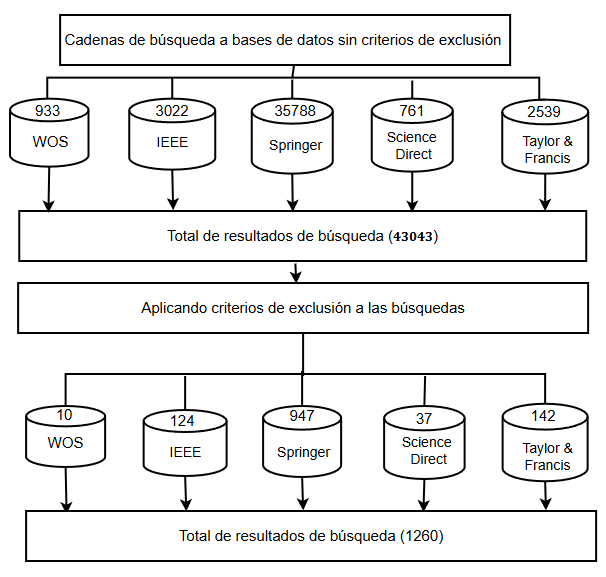
\includegraphics[scale=0.6] {tablas-images/sms/resumen_busqueda_bases.png}
	\caption{Diagrama resumen del proceso de búsqueda en bases de datos}\label{fig:resumen-busqueda-bases}
\end{figure}

%--------------------------------------------------------------------------------------------------------

\section{Eliminación de duplicados}\label{sec:eliminacionDuplicados}
\noindent
La eliminación de estudios duplicados se efectuó mediante la herramienta de gestión bibliográfica Mendeley. Tras la recopilación 
inicial, todos los artículos fueron importados a dicha plataforma, la cual identificó y eliminó automáticamente las publicaciones 
redundantes. Este proceso resultó en la exclusión de \textbf{tres} artículos duplicados, reduciendo el total de estudio a 1.257. La 
figura~\ref{fig:eliminacion-duplicados} presenta una visualización gráfica de estos resultados.


% FIGURA Eliminación de duplicados
\begin{figure}[H]
	\centering
	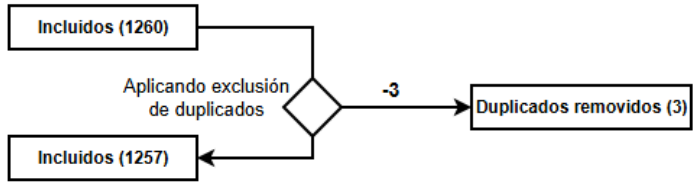
\includegraphics[scale=0.7] {tablas-images/sms/eliminacion-duplicados.png}
	\caption{Diagrama del proceso de eliminación de resultados}\label{fig:eliminacion-duplicados}
\end{figure}

%--------------------------------------------------------------------------------------------------------

\section{Priorización de estudios}\label{sec:priorizacionEstudios}
\noindent


Luego de la selección inicial de los artículos, se realizó una revisión con el nombre de \textit{screening}, este 
procedimiento consiste en verificar \textit{title}, \textit{abstract} y \textit{keywords} de cada uno. Como resultado de esta 
revisión se generaron métricas de calidad para cada artículo, con el fin de priorizar aquellos más relevantes para la investigación. 
Las métricas utilizadas fueron las siguientes:

\begin{itemize}
	\item \textbf{SCI} \textit{(Science Citation Index)}
	\item \textbf{CVI} \textit{(Core Value Index)}
	\item \textbf{IRRQ} \textit{(Index Relation Research Question)}
\end{itemize}
\noindent

Este proceso inició con un total de 1.257 artículos, los cuales fueron evaluados según su alineamiento con los objetivos de la 
investigación. El proceso de \textit{screening} permitió descartar 1.091 estudios dado que algunos hacían referencia a metodologías y  
herramientas tecnológicas de contextos diferentes y otros no estaban alineados con los objetivos de investigación planteados.

Por lo tanto, se terminó la primera estrategia de búsqueda con un total de 166 estudios con una relación directa con el enfoque 
planteado.

%-----------------------------------------------------------------------------------------------------------------------------

\section{Estrategia de búsqueda usando bola de nieve}\label{sec:bolaDeNieve}
\noindent

En esta etapa, la estrategia de búsqueda mediante \textit{snowballing} se aplicó sobre la totalidad de los 166 estudios seleccionados 
tras el proceso de selección, en lugar de emplear un conjunto reducido de artículos base (semilla). Esta decisión permitió ampliar 
la cobertura de la revisión y disminuir el riesgo de omitir literatura relevante, fortaleciendo la exhaustividad del protocolo. En 
este proceso, se aplicaron las estrategias de bola de nieve directa \textit{(Forward)} e inversa con el objetivo de identificar literatura adicional 
relevante que no hubiera sido recuperada durante la búsqueda automática en las bases de datos. En la búsqueda por bola de nieve 
directa se obtuvieron 7 estudios nuevos, mientras que la búsqueda por bola de nieve inversa se obtubieron 8 estudios nuevos, lo que 
resultó en un total de 15 estudios adicionales. El resumen de este proceso puede verse en la figura~\ref{fig:resumen-snowball}

\begin{figure}[H]
	\begin{center}
		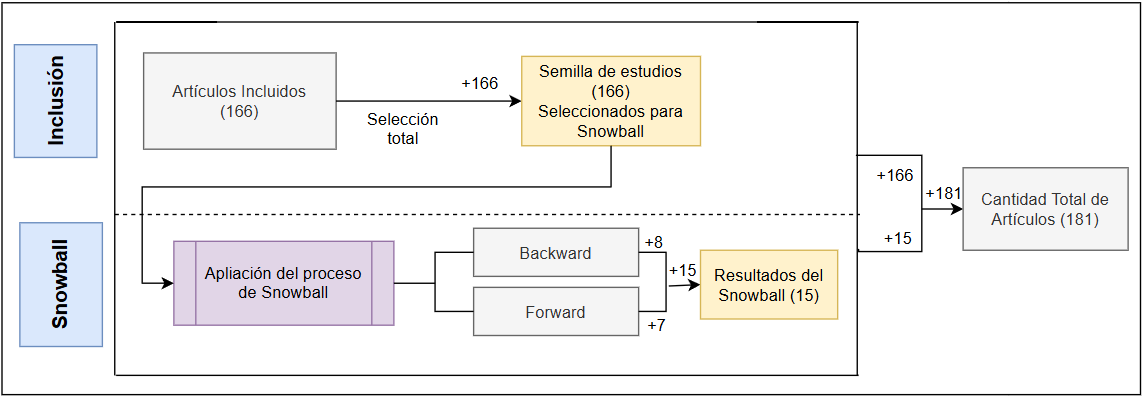
\includegraphics[width=1.0\textwidth]{tablas-images/sms/proceso_snowball2.png}
	\end{center}
	\caption{Resumen del proceso de búsqueda por bola de nieve}\label{fig:resumen-snowball}
\end{figure}

%-----------------------------------------------------------------------------------------------------------------------------

\section{Identificación de estudios}

\section{Cuadro de estudios}

Los estudios resultantes del proceso de \SMS se presentan en la tabla~\ref{table:selected_primary_studies}.


% -------- Tabla : Estudios Primarios Seleccionados (SPSs) ------------
\begin{table}[H]
	\centering
	\fontsize{8pt}{10pt}\selectfont % Tamaño de fuente 8pt
	\renewcommand{\arraystretch}{1.2}
	\begin{tabular*}{\textwidth}{l @{\extracolsep{\fill}} r l @{\extracolsep{\fill}} r l @{\extracolsep{\fill}} r l @{\extracolsep{\fill}} r l @{\extracolsep{\fill}} r}
		\toprule
		\textbf{ID} & \textbf{Ref}                        & \textbf{ID} & \textbf{Ref}                        & \textbf{ID} & \textbf{Ref}                      & \textbf{ID} & \textbf{Ref}                        & \textbf{ID} & \textbf{Ref}                       \\
		\midrule
		SPS001      & \spsone                             & SPS002      & \spstwo                             & SPS003      & \spsthree                         & SPS004      & \spsfour                            & SPS005      & \spsfive                           \\
		SPS006      & \spssix                             & SPS007      & \spsseven                           & SPS008      & \spseight                         & SPS009      & \spsnine                            & SPS010      & \spsten                            \\
		SPS011      & \spseleven                          & SPS012      & \spstwelve                          & SPS013      & \spsthirteen                      & SPS014      & \spsfourteen                        & SPS015      & \spsfifteen                        \\
		SPS016      & \spssixteen                         & SPS017      & \spsseventeen                       & SPS018      & \spseighteen                      & SPS019      & \spsnineteen                        & SPS020      & \spstwenty                         \\
		SPS021      & \spstwentyone                       & SPS022      & \spstwentytwo                       & SPS023      & \spstwentythree                   & SPS024      & \spstwentyfour                      & SPS025      & \spstwentyfive                     \\
		SPS026      & \spstwentysix                       & SPS027      & \spstwentyseven                     & SPS028      & \spstwentyeight                   & SPS029      & \spstwentynine                      & SPS030      & \spsthirty                         \\
		SPS031      & \spsthirtyone                       & SPS032      & \spsthirtytwo                       & SPS033      & \spsthirtythree                   & SPS034      & \spsthirtyfour                      & SPS035      & \spsthirtyfive                     \\
		SPS036      & \spsthirtysix                       & SPS037      & \spsthirtyseven                     & SPS038      & \spsthirtyeight                   & SPS039      & \spsthirtynine                      & SPS040      & \spsforty                          \\
		SPS041      & \spsfortyone                        & SPS042      & \spsfortytwo                        & SPS043      & \spsfortythree                    & SPS044      & \spsfortyfour                       & SPS045      & \spsfortyfive                      \\
		SPS046      & \spsfortysix                        & SPS047      & \spsfortyseven                      & SPS048      & \spsfortyeight                    & SPS049      & \spsfortynine                       & SPS050      & \spsfifty                          \\
		SPS051      & \spsfiftyone                        & SPS052      & \spsfiftytwo                        & SPS053      & \spsfiftythree                    & SPS054      & \spsfiftyfour                       & SPS055      & \spsfiftyfive                      \\
		SPS056      & \spsfiftysix                        & SPS057      & \spsfiftyseven                      & SPS058      & \spsfiftyeight                    & SPS059      & \spsfiftynine                       & SPS060      & \spssixty                          \\
		SPS061      & \spssixtyone                        & SPS062      & \spssixtytwo                        & SPS063      & \spssixtythree                    & SPS064      & \spssixtyfour                       & SPS065      & \spssixtyfive                      \\
		SPS066      & \spssixtysix                        & SPS067      & \spssixtyseven                      & SPS068      & \spsixtyeight                     & SPS069      & \spssixtynine                       & SPS070      & \spsseventy                        \\
		SPS071      & \spsseventyone                      & SPS072      & \spsseventytwo                      & SPS073      & \spsseventythree                  & SPS074      & \spsseventyfour                     & SPS075      & \spsseventyfive                    \\
		SPS076      & \spsseventysix                      & SPS077      & \spsseventyseven                    & SPS078      & \spsseventyeight                  & SPS079      & \spsseventynine                     & SPS080      & \spseighty                         \\
		SPS081      & \spseightyone                       & SPS082      & \spseightytwo                       & SPS083      & \spseightythree                   & SPS084      & \spseightyfour                      & SPS085      & \spseightyfive                     \\
		SPS086      & \spseightysix                       & SPS087      & \spseightyseven                     & SPS088      & \spseightyeight                   & SPS089      & \spseightynine                      & SPS090      & \spsninety                         \\
		SPS091      & \spsninetyone                       & SPS092      & \spsninetytwo                       & SPS093      & \spsninetythree                   & SPS094      & \spsninetyfour                      & SPS095      & \spsninetyfive                     \\
		SPS096      & \spsninetysix                       & SPS097      & \spsninetyseven                     & SPS098      & \spsnineyeight                    & SPS099      & \spsninetynine                      & SPS100      & \spsonehundred                     \\
		SPS101      & \spsonehundredone                   & SPS102      & \spsonehundredtwo                   & SPS103      & \spsonehundredthree               & SPS104      & \spsonehundredfour                  & SPS105      & \spsonehundredfive                 \\
		SPS106      & \spsonehundredsix                   & SPS107      & \spsonehundredseven                 & SPS108      & \spsonehundredeight               & SPS109      & \spsonehundrednine                  & SPS110      & \spsonehundredten                  \\
		SPS111      & \spsonehundredeleven                & SPS112      & \spsonehundredtwelve                & SPS113      & \spsonehundredthirteen            & SPS114      & \spsonehundredfourteen              & SPS115      & \spsonehundredfifteen              \\
		SPS117      & \spsonehundredseventeen             & SPS118      & \spsonehundredeighteen              & SPS119      & \spsonehundrednineteen            & SPS120      & \spsonehundredtwenty        		& SPS121      & \spsonehundredtwentyone            \\
		SPS122 		& \spsonehundredtwentytwo      		  & SPS123 		& \spsonehundredtwentythree    		  & SPS124 		& \spsonehundredtwentyfour    		& SPS125 	  & \spsonehundredtwentyfive    		& SPS126 	  & \spsonehundredtwentysix     	   \\
		SPS127 		& \spsonehundredtwentyseven    		  & SPS128 		& \spsonehundredtwentyeight    		  & SPS129 		& \spsonehundredtwentynine    		& SPS130 	  & \spsonehundredthirty        		& SPS131 	  & \spsonehundredthirtyone     		\\
		SPS132 		& \spsonehundredthirtytwo      		  & SPS133 		& \spsonehundredthirtythree    		  & SPS134 		& \spsonehundredthirtyfour    		& SPS135 	  & \spsonehundredthirtyfive    		& SPS136 	  & \spsonehundredthirtysix     		\\
		SPS137 		& \spsonehundredthirtyseven    		  & SPS138 		& \spsonehundredthirtyeight    		  & SPS139 		& \spsonehundredthirtynine    		& SPS140 	  & \spsonehundredforty         		& SPS141 	  & \spsonehundredfortyone      		\\
		SPS142 		& \spsonehundredfortytwo       		  & SPS143 		& \spsonehundredfortythree     		  & SPS144 		& \spsonehundredfortyfour     		& SPS145 	  & \spsonehundredfortyfive     		& SPS146 	  & \spsonehundredfortysix      		\\
		SPS147 		& \spsonehundredfortyseven     		  & SPS148 		& \spsonehundredfortyeight     		  & SPS149 		& \spsonehundredfortynine     		& SPS150 	  & \spsonhundredfifty        			& SPS151 	  & \spsonehundredfiftyone      		\\
		SPS152 		& \spsonehundredfiftytwo       		  & SPS153 		& \spsonehundredfiftythree     		  & SPS154 		& \spsonehundredfiftyfour     		& SPS155 	  & \spsonehundredfiftyfive     		& SPS156 	  & \spsonehundredfiftysix      		\\
		SPS157 		& \spsonehundredfiftyseven     		  & SPS158 		& \spsonehundredfiftyeight     		  & SPS159 		& \spsonehundredfiftynine     		& SPS160 	  & \spsonehundredsixty         		& SPS161 	  & \spsonehundredsixtyone      		\\
		SPS162 		& \spsonehundredsixtytwo       		  & SPS163 		& \spsonehundredsixtythree     		  & SPS164 		& \spsonehundredsixtyfour     		& SPS165 	  & \spsonehundredsixtyfive     		& SPS166 	  & \spsonehundredsixtysix      		\\
		SPS167 		& \spsonehundredsixtyseven     		  & SPS168 		& \spsonehundredsixtyeight     		  & SPS169 		& \spsonehundredsixtynine     		& SPS170 	  & \spsonehundredseventy      			& SPS171 	  & \spsonehundredseventyone    		\\
		SPS172 		& \spsonehundredseventytwo     		  & SPS173 		& \spsonehundredseventythree   		  & SPS174 		& \spsonehundredseventyfour   		& SPS175 	  & \spsonehundredseventyfive   		& SPS176 	  & \spsonehundredseventysix    		\\
		SPS177 		& \spsonehundredseventyseven   		  & SPS178 		& \spsonehundredseventyeight   		  & SPS179 		& \spsonehundredseventynine   		& SPS180 	  & \spsonehundredeighty        		& SPS181 	  & \spsonehundredeightyone     		\\
		\bottomrule
	\end{tabular*}
	\caption{Los 181 estudios primarios seleccionados (SPSs)}\label{table:selected_primary_studies}
	\vspace{5pt}
\end{table}

%  --------------------------------------------------------------


\subsection{Artículos por año y métricas}
\noindent
A continuación se presentan las gráficas de los resultados de la búsqueda. En la figura~\ref{fig:plot-anios-vs-indices-calidad} se 
muestra el gráfico con la distribución anual de los estudios primarios seleccionados, junto con los resultados de los índices de 
calidad definidas en la sección~\ref{sec:priorizacionEstudios}. Se observa una tendencia creciente en la producción científica entre 
2022 y 2025, con un pico alto en el año 2025, año en el que se concentra la mayor cantidad de estudios incluidos en el análisis.

\begin{figure}[H]
	\begin{center}
		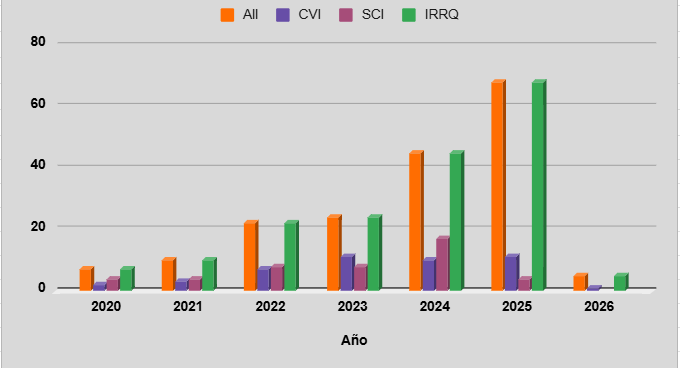
\includegraphics[width=0.6\textwidth]{tablas-images/sms/SPSs_año.png}
	\end{center}
	\caption{Cantidad de artículos en conformidad con las métricas de calidad definidas en~\ref{sec:priorizacionEstudios}}\label{fig:plot-anios-vs-indices-calidad}
\end{figure}

%------------------------------------------------------------------------------------------------------------------------
\subsection{Diferencias entre estrategias}

En la figura~\ref{fig:plot-estrategia_vs_articulos} se pude apreciar la cantidad de artículos obtenido por cada estrategia.

\begin{figure}[H]
	\centering
	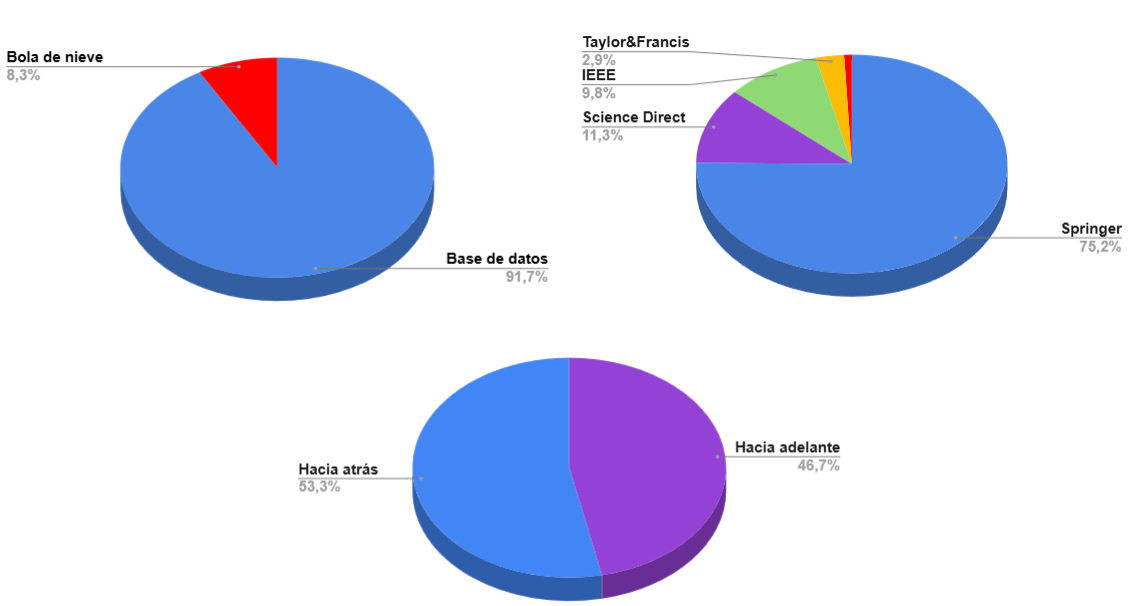
\includegraphics[scale=0.4] {tablas-images/sms/procedencia_datos.png}
	\caption{Diagrama del proceso de eliminación de resultados}\label{fig:plot-estrategia_vs_articulos}
\end{figure}

%------------------------------------------------------------------------------------------------------------------------
\subsection{Promedio de índices de calidad por año}
\noindent

En la figura~\ref{fig:plot-indices} se muestra el promedio anual de los índices de calidad para el conjunto de 181 estudios analizados. 
Se observa que el promedio se mantiene relativamente estable entre 2022 y 2024, con valores cercanos a 1.8–2.0. Sin embargo, en los 
años más recientes que son 2025 y 2026 se observa una disminución moderada, posiblemente debido a que estos estudios aún no cuentan 
con suficiente validación académica o número de citas, lo cual impacta principalmente el índice SCI.\@

Por otro lado, el índice CVI presenta valores estables entre 0.32 y 0.54, lo que indica que el contenido de los estudios se mantiene 
relevante respecto al tema analizado. Asimismo, el índice IRRQ conserva el valor de 1.0 en todos los años, evidenciando una alta 
consistencia entre los estudios seleccionados y las preguntas de investigación.

\begin{figure}[H]
	\centering
	\includegraphics[scale=0.5] {tablas-images/sms/promedio_indices.png}
	\caption{Diagrama del proceso de eliminación de resultados}\label{fig:plot-indices}
\end{figure}

%------------------------------------------------------------------------------------------------------------------------
\subsection{Conformidad con las preguntas de investigación}

Los resultados de la Figura~\ref{fig:terminos} muestran que la investigación se orienta principalmente al desarrollo de metodologías 
y marcos conceptuales en seguridad en la nube, mientras que los estudios centrados en herramientas tecnológicas específicas son 
significativamente menos frecuentes, lo que representa una oportunidad para futuras investigaciones.

El análisis de las categorías que dieron origen a la cadena de búsqueda evidencia que el 53,3\% de los estudios se enfoca en aspectos 
metodológicos y el 44,9\% en el dominio de la seguridad en la nube. En contraste, la categoría relacionada con herramientas 
tecnológicas presenta solo un 1,8\%, lo que confirma una clara predominancia de enfoques conceptuales sobre el desarrollo de 
soluciones tecnológicas específicas.

\begin{figure}[H]
	\centering
	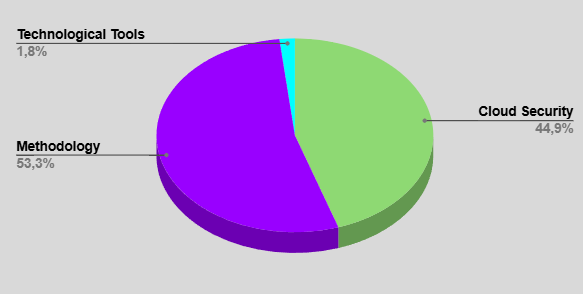
\includegraphics[scale=0.6] {tablas-images/sms/terminos.png}
	\caption{Diagrama del proceso de eliminación de resultados}\label{fig:terminos}
\end{figure}

%------------------------------------------------------------------------------------------------------------------------
\subsection{Taxonomía}

A partir de estos hallazgos, se construyó la taxonomía presentada en la Figura~\ref{fig:taxonomia} la cual permite comprender las 
relaciones entre los enfoques metodológicos, las tecnologías empleadas y los escenarios de aplicación, proporcionando una visión 
estructurada del dominio de la seguridad en la nube. 

La taxonomía se estructura en tres dimensiones principales: tipo de contribución, enfoque de seguridad y contexto de aplicación. 
La dimensión de tipo de contribución agrupa tópicos como computación en la nube, taxonomía, seguridad, arquitectura y controles de 
seguridad. Por su parte, la dimensión de enfoque de seguridad incluye elementos como Zero Trust, sistemas SIEM, normas ISO/IEC 27001, 
ciberseguridad y controles de seguridad. Finalmente, la dimensión de contexto de aplicación organiza los principales escenarios 
identificados en la literatura, incluyendo computación en la nube, arquitectura, seguridad y taxonomía.

Esta organización permite 
\begin{figure}[H]
	\centering
	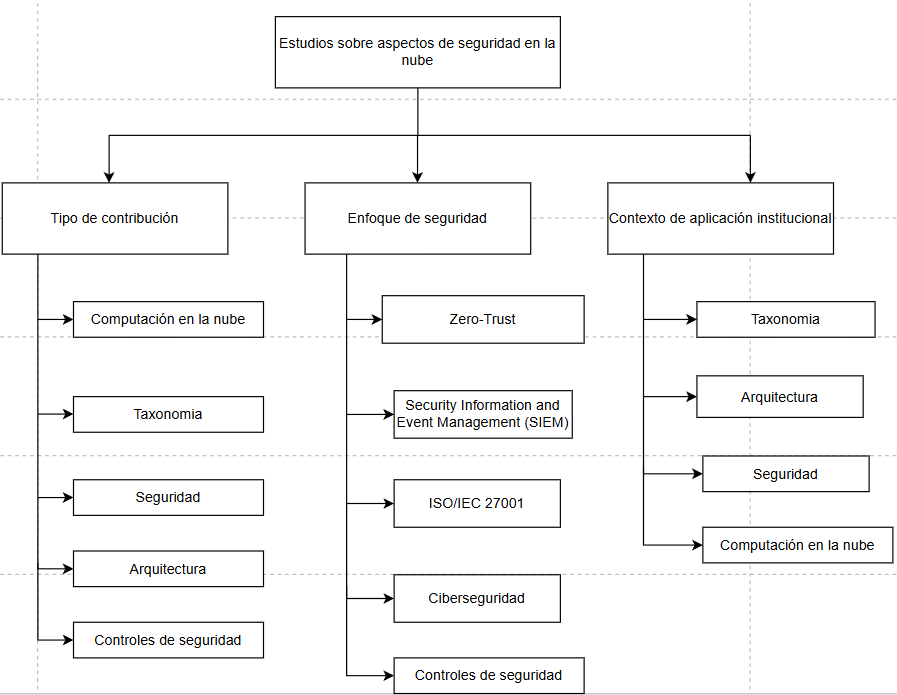
\includegraphics[scale=0.5] {tablas-images/sms/taxonomia.png}
	\caption{Taxonomía de los tópicos identificados en el \SMS}\label{fig:taxonomia}
\end{figure}

%---------------------------------------------------------------------------------------------------------------------------------

\section{Información de la herramienta}

\noindent
La herramienta utilizada para este proceso de revisión de la literatura fue \textbf{SMS-BUILDER}, desarrollada por el Dr.
Christian Andres Candela Uribe la cual se encuentra disponible en \textit{Docker Hub}. La imagen puede consultarse en el 
siguiente enlace:

\begin{center}
	\href{https://hub.docker.com/r/griduq/sms-builder}{\texttt{https://hub.docker.com/r/griduq/sms-builder}}
\end{center}

%----------------------------------------------------------------------------------------------------------------------------
\section{Reproducibilidad del método}
\noindent
Con el fin de fomentar la reproducibilidad del método de revisión, se proporcionan el mecanismo de verificación que permite a los 
revisores y lectores acceder de forma transparente a la información utilizada, generada mediante la herramienta SMS-Builder 
de~\cite{SMSBuilder2020}

\begin{itemize}
	\item Imagen Docker disponible públicamente que integra toda la documentación necesaria para crear un contenedor con los datos del proceso:
 	\url{https://hub.docker.com/r/miguel2409/sms_cloud_security_tg}.
\end{itemize}

\noindent
Adicionalmente, se implementaron procesos de respaldo como medida de seguridad. Estos \textit{backups} fueron almacenados en 
ubicaciones diferentes, siguiendo la estrategia de respaldo \textbf{3--2--1}.

%---------------------------------------------------------------------------------------------------------------------------------
\section{Conclusiones de la revisión sistemática de la literatura}
\noindent
El estudio de mapeo sistemático permitió analizar 181 estudios primarios, identificando las principales tendencias en seguridad en 
la computación en la nube. Los resultados evidencian una predominancia de enfoques metodológicos y el uso recurrente de tecnologías 
como SIEM, Zero Trust y sistemas de detección de intrusiones.

Asimismo, se observó una limitada integración de estos enfoques dentro de arquitecturas unificadas, lo que representa una oportunidad 
para el desarrollo de soluciones más completas y adaptadas a contextos específicos.

En este sentido, el SMS proporcionó una base teórica sólida que respalda la construcción de la arquitectura de seguridad propuesta en 
este trabajo, permitiendo fundamentar la selección de metodologías y tecnologías en evidencia científica actualizada.
